\newpage
\subsection{Caso d'uso UC6: Ricerca API}
\label{UC6}
\begin{figure}[ht]
	\centering
	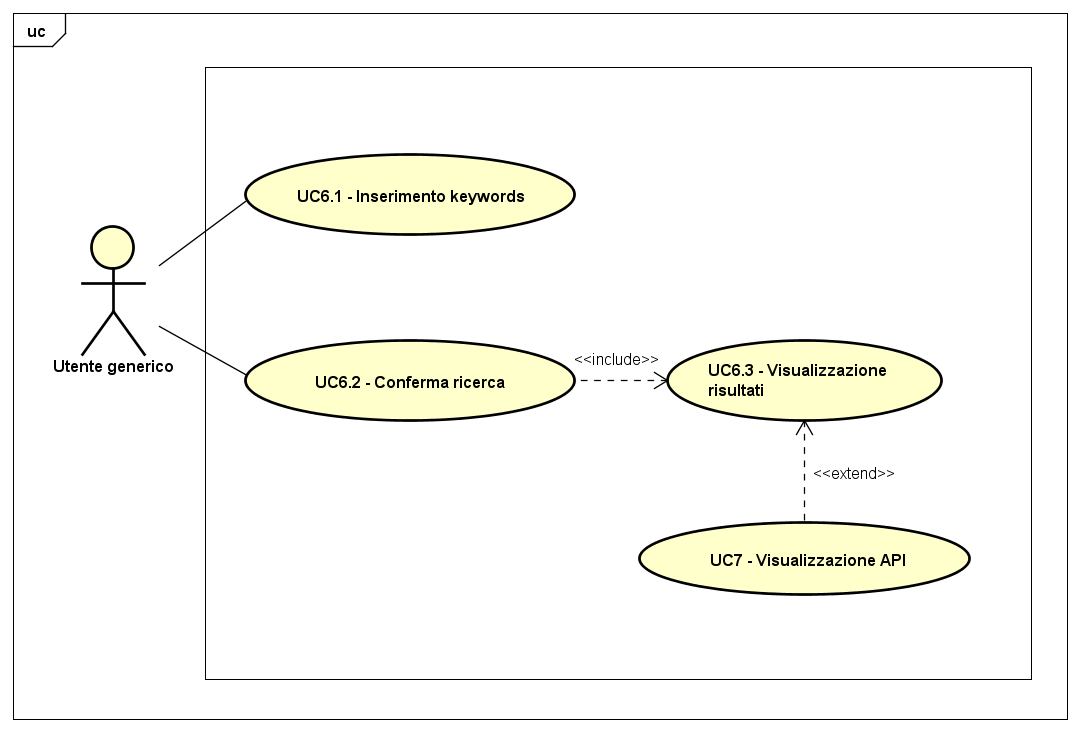
\includegraphics[scale=0.45]{UML/UC6.png}
	\caption{UC6: Ricerca API}
\end{figure}

\begin{longtable}{ l | p{11cm}}
	\hline
	\rowcolor{Gray}
	 \multicolumn{2}{c}{UC6 - Ricerca API} \\
	 \hline
	\textbf{Attori} & Utente generico, Utente non autenticato, Utente autenticato, Amministratore API Market \\
	\textbf{Descrizione} & L'attore inserisce le keywords per la ricerca di API \\
	\textbf{Pre-Condizioni} & L'attore ha scelto di effettuare una ricerca di API \\
	\textbf{Post-Condizioni} & L'attore ha effettuato la ricerca di API ed ha visualizzato la lista dei risultati \\
	\textbf{Scenario Principale} & 
	\begin{enumerate*}[label=(\arabic*.),itemjoin={\newline}]
		\item L'attore può inserire la stringa di ricerca desiderata (UC6.1)
		\item L'attore può confermare i dati inseriti (UC6.2) e visualizzare i risultati forniti dall'applicazione web (UC6.3)
	\end{enumerate*}\\
\end{longtable}